\section{Linear}
\label{sect:linear}

Linear models assume linear dependencies between inputs and outputs, making them among the simplest machine learning approaches. However, their simplicity often results in poor performance in scenarios with significant nonlinear dynamics, such as NBA games \ref{sect:NBA} or soccer games \ref{sect:SOC}. In these domains, more complex models generally outperform linear models, justifying their added complexity. Nevertheless, in cases where the data exhibits more linear characteristics or where the relationships between variables are straightforward, linear models may still provide competitive performance. Therefore, the linear model will be the first and simplest baseline model. It is defined as:

\begin{equation}
    y = W_{xy}x + b_y
\end{equation}

where \( x \) is the input, \( W \) is the weight matrix, \( b \) is the bias, and \( y \) is the output.

\todo{smaller picture \ref{fig:linear-layer}}
\begin{figure}[t]
    \centering
    \includegraphics[width=\textwidth]{contents/Basics/linear.png}
    \caption{Illustration of the internal behavior of a linear layer.}
    \label{fig:linear-layer}
\end{figure}

 This relationship is graphically illustrated in Figure \ref{fig:linear-layer}.

\section{Recurrent}
\label{sect:rnn}

Recurrent models, specifically \gls{rnn}, are designed to handle sequential data effectively. Unlike linear models, \glspl{rnn} have the capability to retain information from previous inputs, making them well-suited for tasks involving \gls{ts} data, \gls{nlp}, and other domains where context is important.

\glspl{rnn} maintain a hidden state, which acts as the memory of the cell. It is updated at each time step using the current input and the previous hidden state. This allows RNNs to capture temporal dependencies and patterns in sequential data. Due to their recurrent nature, they can handle varying sequence lengths unlike linear layers. Figure \ref{fig:rnn} illustrates the internal behavior of an \gls{rnn}, highlighting how these models process and retain sequential information. The recurrent update of the hidden state \( h_t \) and output \( y_t \) at time step \( t \) in an RNN is defined as:

\begin{equation}
    h_t = \sigma(W_{hh} h_{t-1} + W_{xh} x_t + b_h) 
\end{equation}

\begin{equation}
    y_t = W_{hy} h_t + b_y 
\end{equation}

where \( x_t \) is the input at time step \( t \), \( W \) are the weight matrices, \( b \) are the biases, and \( \sigma \) is an activation function, typically a non-linear function like \gls{tanh} or \gls{relu}. The initial hidden state \( h_0 \) is typically initialized to zeros (\( h_0 = \mathbf{0} \)). Sigma is typically a non-linear function, such as sigmoid or \gls{tanh}, chosen for its ability to prevent saturation at extreme values and introduce non-linear behavior. The reason for this choise lies in the saturation of extreme values and providing non-linear behavior. 

Although \glspl{rnn} are appealing due to their ability to handle sequential data, they suffer from drawbacks. One major issue is the vanishing and exploding gradients problem, which causes the model to lose information over time. \gls{lstm} (see Section \ref{sect:lstm}) and \gls{lmu} (see Section \ref{sect:lmu}) are designed to mitigate this issue. Another drawback of \glspl{rnn} is their slow training times. Transformer models (see Section \ref{sect:trafo}) address this by introducing attention heads, which enables training parallelism and also eliminates the \gls{vgp}.

\todo{bigger font}
\begin{figure}[t]
    \centering
    \includegraphics[width=\textwidth]{contents/Basics/rnn_flat.png}
    \caption{Illustration of the internal behavior of a Recurrent Neural Network (RNN).}
    \label{fig:rnn}
\end{figure}

\subsection{Long Short-Term Memory}
\label{sect:lstm}
The \gls{lstm} is a well-established state-of-the-art model in various machine learning applications. It addresses the \gls{vgp} through several gating mechanisms. The \gls{lstm} introduces three primary gates: the input gate, the output gate, and the forget gate. In addition, the cell state is updated by the cell gate mechanism, which plays a distinctive role in integrating new information. Each gate and the cell state work together to control the internal behavior of the modified \gls{rnn} cell. 

The forget gate regulates the flow of information from previous hidden and cell states. The input gate filters essential information from new input data, while the output gate selects pertinent output information. The cell gate, while not traditionally grouped with the primary gates, updates the cell state by integrating filtered new information.

Figure \ref{fig:lstm} illustrates the internal behavior of the \gls{lstm}, depicting how these gates and the cell state interact within the network. Additionally, the following equations define the version of the \gls{lstm} used in the Pytorch Documentation \cite{lstm-pytorch2} and also in :

\begin{equation}
    i_t = \sigma(W_{xi} x_t + W_{hi} h_{t-1} + b_{i})
\end{equation}
\begin{equation}
    f_t = \sigma(W_{xf} x_t + W_{hf} h_{t-1} + b_{f})
\end{equation}
\begin{equation}
    g_t = \tanh(W_{xg} x_t + W_{hg} h_{t-1} + b_{g})
\end{equation}
\begin{equation}
    o_t = \sigma(W_{xo} x_t + W_{ho} h_{t-1} + b_{o})
\end{equation}
\begin{equation}
    c_t = f_t \odot c_{t-1} + i_t \odot g_t
\end{equation}
\begin{equation}
    h_t = o_t \odot \tanh(c_t)
\end{equation}

In these equations, \(i_t\) represents the input gate activation at time step \(t\), while \(f_t\) denotes the forget gate activation at the same time step. The candidate cell state is captured by \(g_t\), and the output gate activation is represented by \(o_t\). The cell state at time step \(t\) is denoted as \(c_t\), and the hidden state as \(h_t\). The input at time step \(t\) is indicated by \(x_t\). The functions \(\sigma\) and \(\tanh\) refer to the sigmoid and \gls{tanh} activation functions, respectively, with \(\odot\) symbolizing element-wise multiplication.

\todo{replace mult with $\odot$ in Figure \ref{fig:lstm}}
\begin{figure}[t]
    \centering
    \includegraphics[width=\textwidth]{contents/Basics/lstm.png}
    \caption{Illustration of the internal behavior of the LSTM.}
    \label{fig:lstm}
\end{figure}


\subsection{Legendre Memory Unit}
\label{sect:lmu}

A novel gateless approach to address gradient vanishing was proposed by Voelker et al. \cite{lmu}. They introduced a method to emulate behaviors observed in the hippocampus, striatum, and cortex of the brain. Similar to these structures, the \gls{lmu} filters information continuously over time. It is claimed to preserve more information over longer durations than \glspl{lstm}, making it a promising alternative layer.

To understand the operation of \gls{lmu}, familiarity with \glspl{lp} is essential. \glspl{lp} are employed to enable the memory state of \gls{lmu} to retain information across extended periods. This requires using an orthogonal polynomial basis. Voelker et al. chose \glspl{lp} because they allow the memory state to be decomposed in a unique way, efficiently capturing long-term dependencies. They approximate the continuous-time delay \( F(s) = e^{-\theta s} \) with a window length \( \theta \) and Laplacian frequency \( s \) using the following ordinary differential equation:

\begin{equation}
\label{eq:ode_approx}
    \theta \dot{m}(t) = Am(t) + B(t)u(t)
\end{equation}

Here, \( m \in \mathbb{R}^d \) (with \( d \) as the memory size) represents the memory state, and \( u \in \mathbb{R} \) is the input, represented in terms of \glspl{lp}. Specifically, it involves sliding windows represented by \glspl{lp} up to degree \( d-1 \). The matrices \( A \in \mathbb{R}^{d \times d} \) and \( B \in \mathbb{R}^{d} \) in Equation \eqref{eq:ode_approx} are defined as:

\begin{equation}
\label{eq:a_bar}
    A = [a]_{ij}, \quad a_{ij} = \begin{cases}
    -1 & \text{if } i < j \\
    (-1)^{i-j+1} & \text{if } i \geq j
    \end{cases}
\end{equation}
\begin{equation}
\label{eq:b_bar}
    B = [b]_i, \quad b_i = (2i + 1)(-1)^i, \quad i, j \in [0, d-1]
\end{equation}

The equation \eqref{eq:ode_approx} is discretized as:

\[
m_t = \bar{A}m_{t-1} + \bar{B}u_t
\]

To achieve this, the continuous matrices \( A \) and \( B \) are discretized to obtain \( \bar{A} \) and \( \bar{B} \). Voelker et al. suggested using methods like Euler's method or \gls*{zoh} for sufficiently small \( \theta \). Algorithm \ref{alg:ssm} outlines the process to derive \( \bar{A} \) and \( \bar{B} \) in pseudocode for clarity. Additionally, Gosalci et al. \cite{gosalci} provided a comprehensive summary of the derivation of all functions described in this chapter.


\begin{algorithm}[H]
\caption{StateSpaceMatrices}
\label{alg:ssm}
\KwIn{$memory\_size$, $\theta$, $dt$}
$Q \gets \text{column vector of integers from } 0 \text{ to } memory\_size-1$\;
$R \gets \frac{1}{\theta}(2 Q + 1)$\;

$(i, j) \gets \text{create meshgrid from } Q$\;

$A \gets \text{zero matrix of size } (memory\_size, memory\_size)$\;
\For{each element $(i, j)$ in $A$}{
    \If{$i < j$}{
        $A[i, j] \gets -R[i, j]$\;
    }
    \Else{
        $A[i, j] \gets R[i, j] \cdot (-1)^{(i - j + 1)}$\;
    }
}

$B \gets \text{column vector of size } (memory\_size, 1)$\;
\For{each element $i$ in $B$}{
    $B[i] \gets R[i] \cdot (-1)^i$\;
}

$A\_discrete \gets dt \cdot A + I$\;
$B\_discrete \gets dt \cdot B$\;

\KwOut{$A\_discrete$, $B\_discrete$}
\end{algorithm}



The \gls{lmu} is defined as:
\begin{equation}
    u_t = e_x^T x_t + e_h^T h_{t-1} + e_m^T m_{t-1}
\end{equation}
\begin{equation}
    m_t = \Bar{A} m_{t-1} + \Bar{B} u_t
\end{equation}
\begin{equation}
    h_t = f(W_x x_t + W_h h_{t-1} + W_m m_t)
\end{equation}
In these equations, \(e_x \in \mathbb{R}^{\text{dim}(x),1}\) represents the input encoding vector, \(e_m \in \mathbb{R}^{d,1}\) is the memory encoding vector, and \(e_h \in \mathbb{R}^{n,1}\) denotes the hidden encoding vector. The weight matrices are defined as \(W_x \in \mathbb{R}^{\text{dim}(x),n}\) for the input, \(W_m \in \mathbb{R}^{d,n}\) for the memory, and \(W_h \in \mathbb{R}^{n,n}\) for the hidden state. The coefficients \(\Bar{A}\) and \(\Bar{B}\) are defined in Equations \eqref{eq:a_bar} and \eqref{eq:b_bar}, respectively. The function \(f\) refers to any nonlinearity, such as sigmoid, tanh, or ReLU. The initial states \(h_0\) and \(m_0\) are typically initialized as zero vectors. Figure \ref{fig:lmu} shows the internal behavior of the LMU graphically.


\begin{figure}[t]
    \centering
    \includegraphics[width=\textwidth]{contents/Basics/lmu.png}
    \caption{Illustration of the internal behavior of the LMU. The dashed line is used to differentiate it from the solid lines it intersects.}    
    \label{fig:lmu}
\end{figure}


\section{Attention-Based Transformer}
\label{sect:trafo}
Despite the development of \gls{lstm} and \gls{lmu}, recurrent models still suffered from information leakage over time, necessitating a new approach. A novel advancement in \gls{nlp} is the use of attention-based models, particularly transformer models, which have become pivotal in the field. As of 2024, most \gls{sota} \glspl{llm}, such as OpenAI's GPT \cite{gpt} and Anthropic's Claude \cite{claude}, are closed-source models utilizing attention mechanisms. On the other hand, open-source alternatives include Meta's LLaMa and OPT \cite{llama,opt}, and Big Science's Bloom \cite{bloom}. Each of these models employs different approaches, making it unclear which architecture is the most promising for the task of predicting trajectories.

The original work by Vaswani et al. \cite{transformer} introduced a model comprising multiple encoder and decoder blocks. However, it was found that the decoder block was not suitable for this task. The decoder-only model generates outputs sequentially and aggregates predictions step-by-step, which can lead to cumulative errors through feedback mechanisms. This sequential generation process makes it prone to increasing inaccuracies over time. Consequently, an encoder-only transformer, such as Devlin et al.'s BERT \cite{bert}, is preferred for this task. The encoder-only transformer processes the entire input at once and generates the output in one step, avoiding the error propagation issues seen in decoder-only models. It consists of a positional encoder (see Section \ref{sec:posenc}) followed by multiple sequential encoder blocks (see Section \ref{sec:enc_block}) and concludes with mini-batch normalization (see Section \ref{sec:laynorm}). This structure is illustrated in Figure \ref{fig:transformer}.

\begin{figure}[t]
    \centering
    \includegraphics[width=\textwidth]{contents/Basics/transformer.png}
    \caption{Illustration of the internal behavior of the Transformer.}
    \label{fig:transformer}
\end{figure}

Figure \ref{fig:transformer} provides a high-level view of the Transformer model. The subsequent sections will delve into specific components of the transformer, each accompanied by a detailed illustration and pseudocode.

\subsection{Positional Embeddings}
\label{sec:posenc}
In transformer models, positional embeddings are crucial for incorporating the order of the sequence into the model. Unlike \glspl{rnn} that process sequences step-by-step, transformers process the entire sequence simultaneously. Therefore, they need a mechanism to inject information about the position of each token in the sequence, enabling the model to understand the order and temporal relationships between tokens.

\subsubsection{Importance of Positional Embeddings}

Positional embeddings provide a sense of order to the model, allowing it to distinguish between tokens at different positions in the sequence. They help the model capture temporal dependencies, which is particularly important for sequential data such as text or audio. By knowing the position of each token, the model can better understand the context in which each token appears, improving its ability to generate accurate and contextually relevant outputs.

\subsubsection{Sinusoidal Positional Embeddings}

The original transformer model by Vaswani et al. \cite{transformer} introduces sinusoidal positional embeddings. These embeddings use sine and cosine functions of different frequencies to encode the position of each token in a sequence. The positional encoding for a position $pos$ and dimension $i$ is defined as follows:

\begin{minipage}{\textwidth}
\begin{equation}
\text{PE}_{(pos, 2i)} = \sin\left(\frac{pos}{10000^{\frac{2i}{d_{\text{model}}}}}\right)
\end{equation}
\begin{equation}
\text{PE}_{(pos, 2i+1)} = \cos\left(\frac{pos}{10000^{\frac{2i}{d_{\text{model}}}}}\right)
\end{equation}
\end{minipage}

where $pos$ is the position and $i$ is the dimension index. This approach allows the model to easily learn to attend by relative positions.

\subsubsection{Convolutional Layer as Positional Embedding}

In their work, Baevski et al. \cite{baevski2020} use a convolutional layer instead of sinusoidal positional embeddings. A convolutional layer is utilized for its ability to effectively capture temporal dependencies, which is essential for understanding the structure and content of sequential data such as speech. The convolutional layer is effective at extracting local temporal features, crucial for capturing low-level patterns in the data.

Moreover, rather than using fixed positional embeddings that encode absolute positional information, Baevski et al. employ a convolutional layer as a relative positional embedding. This approach allows the model to encode relative positional information, which can be more flexible and beneficial for various tasks. The output of the convolution is followed by a \gls{gelu} activation and then added to the inputs, followed by layer normalization.

For tasks involving the prediction of trajectories in complex scenes, such as \gls{nba} games or soccer matches, a convolutional layer can offer several advantages. By providing a hierarchical representation of the input, the model can capture both local and broader temporal contexts. This representation can be particularly beneficial for understanding the dynamic and intricate patterns in sports trajectories, where both short-term movements and longer-term strategies need to be considered.

Furthermore, the convolutional layer can reduce the length of the input sequence through pooling or strided convolutions, which reduces computational complexity for the subsequent transformer layers. This can be advantageous in handling the extensive data generated in sports scenarios, allowing for more efficient and scalable model training and inference.



\subsection{Encoder Block}
\label{sec:enc_block}
The Transformer model primarily consists of encoder blocks. Each encoder block processes the input through a series of layers, including \gls{mha} and \glspl{ffn}. The detailed structure of an encoder block is shown in Figure \ref{fig:encoder_block}. The pseudocode for the encoder block forward pass is provided in Algorithm \ref{alg:encoder_layer}.

\begin{figure}[t]
    \centering
    \begin{minipage}{\textwidth}
        \includegraphics[width=\textwidth]{contents/Basics/encoder_block.png}
        \caption{Zoom into the encoder block of the Transformer.}
        \label{fig:encoder_block}
    \end{minipage}
    \vspace{-1em} % Adjust vertical space if necessary
\end{figure}

\todo{Make colors less saturated in Figure \ref{fig:encoder_block}.}

\begin{figure}[t]
    \centering
    \includegraphics[width=\textwidth]{contents/Basics/MHA.png}
    \caption{Zoom into the Multi-Head Attention.}
    \label{fig:multihead_attention}
\end{figure}

\begin{algorithm}[H]
\caption{EncoderLayer Forward Pass}
\label{alg:encoder_layer}
\KwIn{$x$, $encoder\_mask$}
$c1 \gets \text{LayerNorm}_1(x)$\;
$c2 \gets \text{MultiHeadAttention}(c1, c1, c1, encoder\_mask)$\;
$c3 \gets c2 + x$\;
$c4 \gets \text{LayerNorm}_2(c3)$\;
$c5 \gets \text{PositionwiseFFN}(c4)$\;
\KwOut{$c3 + c5$}
\end{algorithm}


In the encoder block, the input $x$ first passes through a Layer Normalization step (see Section \ref{sec:laynorm}). The normalized input, denoted as $c1$, then goes through the \gls{mha} mechanism which is detailed in Section \ref{sec:mha}. The resulting $c2$ is added to the input vector $x$ to get $c3$. $c4$ is then fed through a second Layer Normalization, and after being processed by the \gls{ffn} (see Section \ref{sec:ffn}), we obtain $c5$. The final output of the encoder block is $c3 + c5$.


\subsection{Multi-Head Attention}
\label{sec:mha}
\gls{mha} is a key component of the transformer model, enabling it to focus on different parts of the input sequence simultaneously. In this mechanism, the input is split into multiple heads of size $d_k$. Each head is processed through a linear layer and then fed into the Scaled Dot-Product Attention. The outputs from all heads are concatenated and processed through another linear layer. This detailed structure is shown in Figure \ref{fig:multihead_attention}.

\begin{algorithm}[H]
\caption{Multi-Head Attention Forward Pass}
\label{alg:multihead_attention}
\KwIn{Queries, Keys, Values, Mask}
$d_k \gets \frac{n\_out}{n\_heads}$\;
Queries' $\gets \text{Linear}(\text{Queries})$\;
Keys' $\gets \text{Linear}(\text{Keys})$\;
Values' $\gets \text{Linear}(\text{Values})$\;
Queries $\gets \text{SplitIntoHeads}(\text{Queries', }d_k)$\;
Keys $\gets \text{SplitIntoHeads}(\text{Keys', }d_k)$\;
Values $\gets \text{SplitIntoHeads}(\text{Values', }d_k)$\;
$x \gets \text{ScaledDotProductAttention}(\text{Queries, Keys, Values, Mask})$\;
$x \gets \text{Reshape}(x)$\;
$x \gets \text{Linear}(x)$\;
\KwOut{$x$}
\end{algorithm}

The pseudocode for the \gls{mha} forward pass is provided in Algorithm \ref{alg:multihead_attention}. It illustrates the process of splitting the input into Queries, Keys, and Values heads. These are then processed through the \gls{sdpa} (see Section \ref{sec:sdpa}). After reshaping, the output is obtained by applying a final linear layer.


\subsection{Scaled Dot-Product Attention}
\label{sec:sdpa}

\begin{figure}[t]
    \centering
    \includegraphics[width=0.5\textwidth]{contents/Basics/scaled_dot_product.png}
    \caption{Zoom into the Scaled Dot-Product Attention.}
    \label{fig:scaled_dot_product}
\end{figure}
Within the \gls{mha} mechanism, Scaled Dot-Product Attention is essential for computing the attention scores between queries and keys. These scores are then used to weigh the values. An optional encoder mask can be applied to prevent certain positions from attending to others, though this feature is not used in this work. A detailed view of Scaled Dot-Product Attention is shown in Figure \ref{fig:scaled_dot_product}.

The function of Scaled Dot-Product Attention is mathematically represented as:

\begin{equation}
\text{Attention}(Q, K, V) = \text{softmax}\left(\frac{QK^T}{\sqrt{d_k}}\right)V
\end{equation}

where $Q$, $K$, and $V$ are the query, key, and value matrices, respectively, and $d_k$ is the dimension of the keys.

Softmax is a function used to convert the attention scores into a probability distribution. It ensures that the weights assigned to each key sum to one, allowing the model to interpret these weights as probabilities. The Softmax function is defined as:

\begin{equation}
\text{softmax}(z_i) = \frac{\exp(z_i)}{\sum_{j} \exp(z_j)}
\end{equation}

where \( z_i \) represents the score for the \( i \)-th key, and the denominator sums over all scores to normalize them.

The algorithm for Scaled Dot-Product Attention proceeds as follows: First, the attention scores are computed by taking the dot product of the query matrix $Q$ and the transpose of the key matrix $K$, and then scaling these scores by \( \sqrt{d_k} \). This scaling is crucial to avoid excessively large values in the dot product. The scaled scores are then passed through the Softmax function to obtain normalized attention weights. If an encoder mask is used, it adjusts the attention scores accordingly, though this is not applicable in the current work. Finally, these attention weights are applied to the value matrix $V$ to produce the weighted output. This mechanism enables the model to focus on different parts of the input sequence based on the computed attention weights.


\subsection{Positionwise Feed-Forward Network}
\label{sec:ffn}
After the attention mechanism, the data passes through a \gls{ffn}, which applies a fully connected network to each position independently and identically. The \gls{ffn} consists of two linear layers with a ReLU activation function in between, followed by a dropout layer. The detailed structure of the \gls{ffn} is shown in Figure \ref{fig:ffn} and the pseudocode is provided as Algorithm \ref{alg:ffn2}.

Finally, each encoder block concludes with another Layer Normalization step, ensuring stable and normalized data propagation.

\begin{figure}[t]
    \centering
    \includegraphics[width=\textwidth]{contents/Basics/FeedforwardNetwork.png}
    \caption{Zoom into the Feedforward Mechanism of the encoder.}
    \label{fig:ffn}
\end{figure}

\subsection{Layer Normalization}
\label{sec:laynorm}
Layer normalization is applied to both the input and output of the attention and feed-forward layers. It normalizes the input tensor across the features and is defined as:

\begin{equation}
\label{eq:layernorm}
    y = \frac{x - \text{E}[x]}{\sqrt{\text{Var}[x] + \epsilon}} \cdot \gamma + \beta
\end{equation}

In this equation, \( \text{E}[x] \) represents the mean of the input tensor, while \( \text{Var}[x] \) denotes its variance. The term \( \epsilon \) is a small constant added to the variance to ensure numerical stability. The parameters \( \gamma \) and \( \beta \) are learnable, with \( \gamma \) serving as a scale parameter that adjusts the normalized output, and \( \beta \) acting as a shift parameter that offsets the normalized output.

\begin{algorithm}[H]
\caption{Positionwise Feed-Forward Network Forward Pass}
\label{alg:ffn2}
\KwIn{$x$}
$x \gets \text{Linear}_1(x)$\;
$x \gets \text{ReLU}(x)$\;
$x \gets \text{Dropout}(x)$\;
$x \gets \text{Linear}_2(x)$\;
\KwOut{$x$}
\end{algorithm}


\subsection{Learning Rate-Warm-Up Scheduler}
\label{sec:scheduler}

Training transformer models requires careful selection of the optimizer and learning rate schedule to ensure stable and efficient learning. The Adam \cite{adam} optimizer is commonly used due to its ability to adjust learning rates dynamically for each parameter based on gradient estimates. However, transformers are particularly sensitive to the learning rate, especially in the early stages of training.

To address this, a warm-up phase is introduced, where the learning rate starts low and increases gradually. This prevents large gradient updates from destabilizing the training process in the beginning. The learning rate schedule typically follows the formula proposed by Vaswani et al. \cite{transformer}:

\begin{equation}
\text{LR}(step) = d_{\text{model}}^{-0.5} \cdot \min(step^{-0.5}, step \cdot warmup\_steps^{-1.5})
\end{equation}

Here, $d_{\text{model}}$ is the model’s dimensionality, and $warmup\_steps$ determines the length of the warm-up phase. After the warm-up, the learning rate decreases based on the inverse square root of the step count. This approach ensures that the model trains smoothly, avoiding instability, and achieves better performance by allowing the optimizer to adapt gradually.

For instance, the \gls{llama} \cite{llama} model uses the AdamW optimizer with a linear learning rate warm-up schedule of 2,000 \(warmup\_steps\). Similarly, the \gls{opt} \cite{opt} model also employs AdamW with a linear warm-up of 2,000 \(warmup\_steps\). \gls{bert} \cite{bert} utilizes the Adam optimizer with a warm-up phase of 10,000 \(warmup\_steps\), while \gls{bloom} \cite{bloom} adopts Adam with a cosine learning rate decay schedule.


\section{BitNet: 1-Bit Transformer}
\label{sect:bitnet}

BitNet, as introduced by Wang et al. \cite{BitNet2023}, innovatively replaces the traditional linear layers of the Transformer model with BitLinear layers. This modification involves reducing the precision of weights and activations to 1 bit, thereby significantly decreasing computational and memory requirements. Unlike traditional transformers, BitNet can leverage higher learning rates, enhancing training efficiency.

The core of BitNet's architecture is the BitLinear layer, which employs binary weights and activations. During forward propagation, the computations are performed using bitwise operations, which are inherently faster and more efficient than standard floating-point operations. The output of a BitLinear layer is expressed as:
\[
\mathbf{y} = \text{sign}(\mathbf{W}\mathbf{x} + \mathbf{b})
\]
where \(\mathbf{W}\) and \(\mathbf{x}\) represent the binary weight matrix and input vector, respectively, and \(\mathbf{b}\) denotes the bias term.

The primary advantage of BitNet lies in its substantial reduction of memory and energy consumption. This is particularly beneficial in high dynamic environments where predicting trajectories demands efficient and scalable models. Compared to traditional Transformers, \gls{lstm}, and LMUs, BitNet maintains the effectiveness of the Transformer architecture while optimizing resource usage, leading to a promising modification. Additionally, BitNet allows for larger learning rates compared to Transformers and does not require a warmup phase.

\section{TimeGPT}
\label{sect:timegpt}

TimeGPT was initially identified as a promising tool for time series forecasting due to its precompiled Transformer model specifically designed for time series analysis. The initial availability of TimeGPT as a free resource made it an attractive option for leveraging advanced Transformer-based techniques without financial costs.

However, during the course of the research, TimeGPT transitioned to a subscription-based model, requiring payments of \$99.00 for basic access and \$399.00 for additional support services. This change in the pricing structure significantly impacted its suitability for continued use in the research. The introduction of these fees conflicted with the objective of maintaining a cost-effective and financially independent research framework. Additionally, reliance on a subscription model raised concerns about potential financial benefits accruing to the service provider from the research activities.

Furthermore, there was a strong preference for utilizing and developing open-source solutions. Open-source tools provide transparency, reproducibility of results, and eliminate financial constraints on research activities. This approach ensures the integrity and independence of the research process.

In light of these considerations, TimeGPT was excluded from the research framework. The decision to exclude TimeGPT was motivated by the need to avoid endorsing proprietary software and to prioritize tools that do not benefit financially from the research efforts. The focus was thus redirected towards self-trained models and freely available resources, ensuring that the study remains unbiased and independent.

In conclusion, although TimeGPT initially appeared to be a viable option due to its advanced capabilities and initial free access, the subsequent change in its accessibility and associated costs necessitated its exclusion. This decision underscores the commitment to open-source methodologies and the financial independence of the research.

\section{Performance Measurement}
\label{sec:performance}
\gls{mse} quantifies the average squared difference between predicted and true values. It is defined as:
\begin{equation}
\text{MSE} = \frac{1}{n \cdot m} \sum_{i=1}^n \sum_{j=1}^m \left( \hat{y}_{i,j} - y_{i,j} \right)^2
\end{equation}
where \(\hat{y}_{i,j}\) and \(y_{i,j}\) are the predicted and actual values, respectively, for the \(i\)-th sample and \(j\)-th feature, \(n\) is the number of samples, and \(m\) is the number of features. This meassurement is also used to train the models.

\section{Transfer Learning}
\label{sect:transfer-learning}

\gls{tl} is a technique where knowledge acquired from training a model on one domain is utilized to enhance performance on a different, but related, domain. This method is especially valuable when the target domain has limited data or when it is impractical to train a model from scratch due to high computational costs.

The process of \gls{tl} involves several key steps. Initially, a model is pre-trained on a large and diverse dataset from a source domain. This source dataset allows the model to learn general features and patterns that are broadly applicable. Once pre-training is complete, the model undergoes fine-tuning on a new dataset from the target domain. This step adjusts the model's parameters to better align with the specific characteristics of the target data. Fine-tuning can either involve training the entire model or selectively adjusting certain layers, depending on the degree of similarity between the source and target domains. Finally, the performance of the fine-tuned model is evaluated to ensure that it effectively generalizes to the new domain and meets the desired performance criteria.

\gls{tl} has demonstrated significant effectiveness across various fields. In computer vision, for example, models pre-trained on large image datasets such as ImageNet have been successfully adapted for diverse tasks including object detection and medical image analysis \cite{pan2009survey, GoodBengCour16}. Similarly, in natural language processing, pre-trained models like BERT and GPT have been fine-tuned for specific tasks such as sentiment analysis and translation \cite{bert, radford2019language}.

In this research, \gls{tl} is utilized to investigate whether models trained on basketball data can be effectively adapted and fine-tuned for soccer data and vise versa. This approach aims to evaluate the generalizability of features learned from one sport to another and to assess how well pre-trained models can be adapted to new types of data.
